\section{202109-2 非零段划分}
	\begin{itemize}
		\item 时间限制:$1.0\texttt{ s}$.
		\item 空间限制:$512.0\texttt{ MiB}$.
	\end{itemize}
	\subsection{题目}
		\subsubsection{题目描述}
			\par $A_1, A_2, \cdots, A_n$ 是一个由 $n$ 个自然数(非负整数)组成的数组。我们称其中 $A_i, \cdots, A_j$ 是一个非零段,当且仅当以下条件同时满足:
			\begin{itemize}
				\item $1\leq i\leq j\leq n$;
				\item 对于任意的整数 $k$,若 $i\leq k\leq j$,则 $A_k>0$;
				\item $i=1$ 或 $A_{i-1}=0$;
				\item $j=n$ 或 $A_{j+1}=0$。
			\end{itemize}
			\par 下面展示了几个简单的例子:
			\begin{itemize}
				\item $A = [3, 1, 2, 0, 0, 2, 0, 4, 5, 0, 2]$中的  个非零段依次为 $[3, 1, 2]$、$[2]$、$[4, 5]$ 和 $[2]$;
				\item $A = [2, 3, 1, 4, 5]$ 仅有 $1$ 个非零段;
				\item $A = [0, 0, 0]$ 则不含非零段(即非零段个数为 $0$)。
			\end{itemize}
			\par 现在我们可以对数组 $A$ 进行如下操作:任选一个正整数 $p$,然后将 $A$ 中所有小于 $p$ 的数都变为 $0$。试选取一个合适的 $p$,使得数组 $A$ 中的非零段个数达到最大。若输入的 $A$ 所含非零段数已达最大值,可取 $p=1$,即不对 $A$ 做任何修改。
		\subsubsection{子任务}
			\par $70\%$ 的测试数据满足 $n\leq 1000$;
			\par 全部的测试数据满足 $n\leq 5\times 10^5$,且数组 $A$ 中的每一个数均不超过 $10^4$。
	\subsection{解法 A(70 分)}
		\subsubsection{原理阐释}
			\par 考虑一个朴素的办法,枚举 $p$ 的取值,每次用 $\Theta(n)$ 的时间完成修改操作并统计非零段的个数,考虑到 $A$ 的值域有限,这个方法可以取得不错的速度。
			\par 时间复杂度为 $\Theta(n\left\lvert A\right\rvert)$,空间复杂度为 $\Theta(n)$。
		\subsubsection{C++ 代码实现}
			\lstinputlisting[
				style=C++,
				title={\bf 202109-2-subtask1.cpp}
			]{202109-2-subtask1.cpp}
	\subsection{解法 B(100 分)}
		\subsubsection{原理阐释}
			\par 注意到若 $p+1$ 在 $A$ 中没有出现,则取 $p$ 和取 $p+1$ 后 $A$ 的状态没有改变,从而我们得知只需要处理 $A$ 中出现了的值即可。
			\par 更进一步地,若我们知道了需要修改的值和其在 $A$ 中的位置,我们可以在常数级别的时间内快速维护答案。从而时间复杂度均摊为 $\Theta(n)$。
			\par 总而言之,我们只需要简单维护每一个值出现的位置,并利用其快速维护答案即可。时间复杂度为 $\Theta(n+\left\lvert A\right\rvert)$,空间复杂度为 $\Theta(n+\left\lvert A\right\rvert)$。
		\subsubsection{C++ 代码实现}
			\lstinputlisting[
				style=C++,
				title={\bf 202109-2.cpp},
				tabsize=4
			]{202109-2.cpp}
		\subsubsection{提交结果}
			\begin{figure*}[htbp]
				\centering
				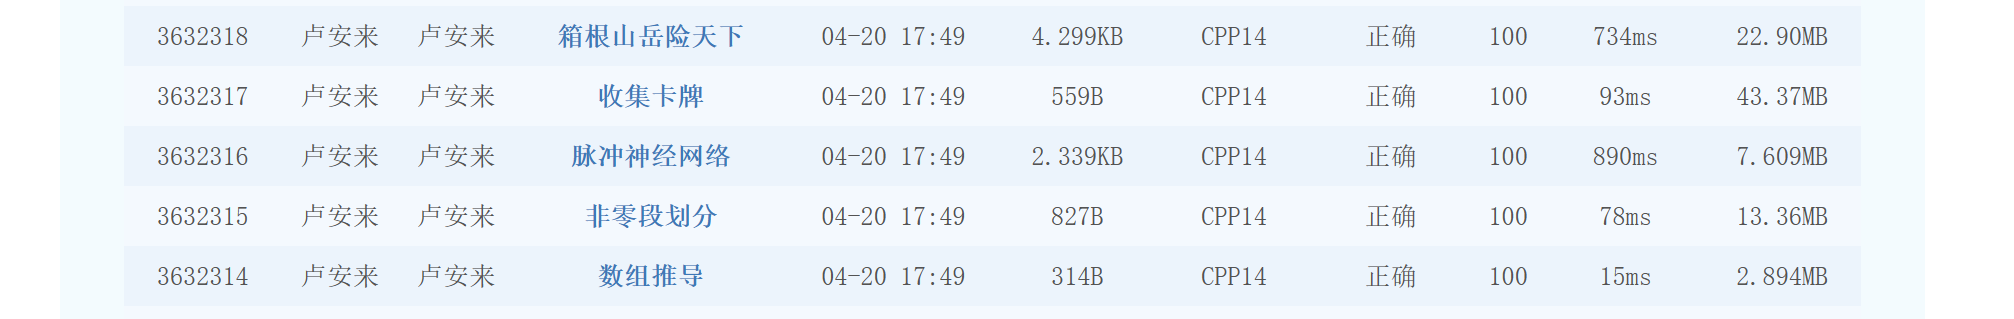
\includegraphics[width=1\textwidth]{result.png}
				\caption{提交结果}
			\end{figure*}